% !TEX encoding = UTF-8
% !TEX TS-program = pdflatex
% !TEX root = ../dev-manual.tex

%**************************************************************
\chapter{DataMole architecture}
\label{ch:arch}
%**************************************************************

\section{Technology}
This section describes the main technologies that were selected to realise DataMole.\\
DataMole was developed in Python in order to maximise interoperability with other packages and to take advantage of the existing data analysis libraries. The main dependencies are listed below:
\begin{itemize}
	\item \textbf{Pandas 1.0.5}: Pandas dataframe is used to manage datasets and its rich API is used in the program to apply transformations and manipulate the data;
	\item \textbf{Scikit-learn 0.23.1}: this library is used to apply some transformations, because of its excellent compatibility with Pandas;
	\item \textbf{Networkx 2.4}: a library for graph management and analysis used to create and manage the computational graph;
	\item \textbf{Numpy 1.19.1}: a library for scientific computing and number crunching;
	\item \textbf{PySide2 5.15.0}: contains the Python bindings of the Qt Framework version 5.15.0 and is used to create the graphic interface;
	\item \textbf{Prettytable 0.7.2}: a library for printing formatted ASCII tables, used with logging;
	\item \textbf{PyTest 5.4.3}: to write tests;
	\item \textbf{Sphinx 3.2.1}: used to automatically generate the documentation for the project.
\end{itemize}

\subsection{Dataset management libraries}\label{ssec:dataset-manag}
Pandas dataframes are used in DataMole to manage datasets, but other libraries offering similar data structures that were taken in consideration and are listed here.
\begin{itemize}
	\item \textbf{Dask}: a project started in 2015 with the goal of creating a distributed computing library with big data support. It offers a dataframe API very similar to Pandas, with the difference of being able to manage huge out-of-memory datasets;
	\item \textbf{Datatable}: a Python porting of the popular \texttt{data.table} package for R, developed by the same authors. Only a beta version is currently released, and many features of the R version are missing. Similarly to the R package it can deal with out-of-memory datasets;
	\item \textbf{PySpark}: a big data computing framework written in Scala which supports data stream, map-reduce operations on distributed file systems;
	\item \textbf{Turicreate}: a project currently maintained by Apple with the goal of simplifying the development of custom machine learning models. It supports big data computations and provides the SFrame container, a scalable dataframe similar to a Pandas dataframe;
	\item \textbf{Modin}: a project with the goal of scaling Pandas to big datasets. Internally is uses Dask or Ray to transparently process dataframes and to support out-of-core and parallel computations.
\end{itemize}
Both \texttt{Spark} and \texttt{Dask} are designed to work with big data and heavy computations: internally they use a scheduler and add complexity to support distributed file systems. This focus on big data often results in additional computational overhead, which is unjustified for the purpose of this project at its current state.\\ 
\texttt{Datatable} and \texttt{turicreate} are much simpler to use than the previous libraries, since they do not handle distributed computation. \texttt{Datatable} main disadvantage is its very limited API with respect to Pandas and the missing support for Windows. \texttt{Turicreate} is more limited then Pandas, but still comes with a rich set of features that makes it probably suitable for this project. It has one limitation: it works only with 64-bit machines. \\
Finally \texttt{Modin} was discarded because it is still an experimental project.\\
Adding big data support is of course desirable, but comes with additional costs and overhead that should be taken into account. With respect to this project objectives, I found the additional complexity not worth it, especially for an initial release, and decided to work with Pandas. This library has also the advantage of being well integrated in the Python ecosystem, and its dataframes are supported by other packages like Scikit-learn. Naturally the other listed libraries may be reconsidered for future extension, if scalability becomes a concern.

\section{Qt basics}
\label{ssec:qt-basics}
This section briefly describes two important features of Qt that have been widely used to develop DataMole. The purpose of this section is not to provide a comprehensive description of the Qt Framework and its functionalities, but merely to clarify the meaning of some technical terms that will often be used throughout this chapter.

\subsection{Signals and slots}
Signals and slots are used for communication between objects and their combined usage represents the Qt approach to event-driven programming \cite{site:qt-doc-signals}.\\
A \textit{signal} is emitted when a particular event occurs. For example when a button is clicked, the \texttt{clicked} signal is emitted. A \textit{slot} is a member function that is called in response to a particular signal. Qt widgets come with many predefined signals and slots, but they can be subclassed to add new customised slots handling specialised signals.

\subsection{Model-view-delegate}
The Qt Framework provides a set of classes that use a model/view architecture to manage the separation between data and the way it is presented to the user \cite{site:qt-doc-model-view}.
This is achieved with the combined usage of three components:
\begin{itemize}
	\item \textit{Model}: model classes inherit \texttt{QAbstractItemModel} that provides an interface for the other components in the architecture. The model communicates with the data: it can hold the data or it can be a proxy between the data container and the other components;
	\item \textit{View}: view classes inherit \texttt{QAbstractItemView} and their instances obtain references to items of data from the model. With these, a view can retrieve items from the data source and display them to the user;
	\item \textit{Delegate}: a delegate renders the items of data inside a view and, when items are edited, it communicates with the model to change its state. Every delegate class inherits \texttt{QAbstractItemDelegate}.
\end{itemize}
These components define the \textit{model-view-delegate} pattern, which is extensively used to show information in DataMole.

\section{Architecture overview}
\label{sec:architecture}
This section describes the architectural choices made while designing the DataMole software architecture. UML class diagrams are presented alongside packages description to model the relation between different components. Moreover, several sequence diagrams are shown in §\ref{sssec:pipeline-sequence} to show the interaction between GUI components that is required to carry out some operations.\\
The extension mechanisms, some implementation details, as well as a detailed description of various classes and their methods, are included in the next chapter.

\subsection{Description of the main packages}
\label{ssec:packages}
DataMole is a Python package, composed of many sub-packages and modules. In Python notation a \textit{module} is a single file containing definitions and statements, while a \textit{package} is a collection of modules (e.g. a directory containing Python files and possibly other packages) \cite{docs:python-mod-pack}. The complete directory structure can be seen later, in §\ref{sec:dirtree}.\\
The main DataMole package, named \texttt{dataMole}, is organised in 4 sub-packages:
\begin{itemize}
	\item \textit{data}: defines the container classes for dataframe objects and everything required for their management. Every Pandas dataframe is wrapped inside \texttt{Frame} object. Every dataframe has a \texttt{Shape}, which is a description of the columns names and their types. Finally a hierarchy of classes was defined to model the supported data types;
	\item \textit{flow}: defines the data structure used to contain the flowgraph (\texttt{OperationDag}) and the handler to execute it in separate threads (\texttt{OperationHandler});
	\item \textit{gui}: contains all the widgets and GUI components used within the software. It is further composed of 4 sub-packages:
	\begin{itemize}
		\item \textit{charts}: contains the widgets used to create and visualise all the charts;
		\item \textit{editor}: defines the abstract class \texttt{AbsOperationEditor}, the super-type of all editor widgets used for operation configuration. It also contains the definition of the editor factory \texttt{OptionsEditorFactory}, defined as a \textit{singleton}, and many utilities to configure the operation and show the operation documentation;
		\item \textit{graph}: collection of components which realise the user interface for the \textit{Flow panel}. It relies on the \textit{Qt Graphics View Framework} and part of the implementation was taken from an existing work available at \cite{site:nodegraph-pyqt};
		\item \textit{widgets}: contains the definition of several widgets used in the program.
	\end{itemize}
	\item \textit{operation}: defines the common super-type of all operations and its subclasses, which model every data transformations;
	\item \textit{flogging}: the DataMole logging module. Also defines the interface to be implemented in every operation whose execution must be logged to file (\texttt{Loggable}).
\end{itemize}

\subsection{Model/view classes}
\begin{figure}[ht]
	\centering
	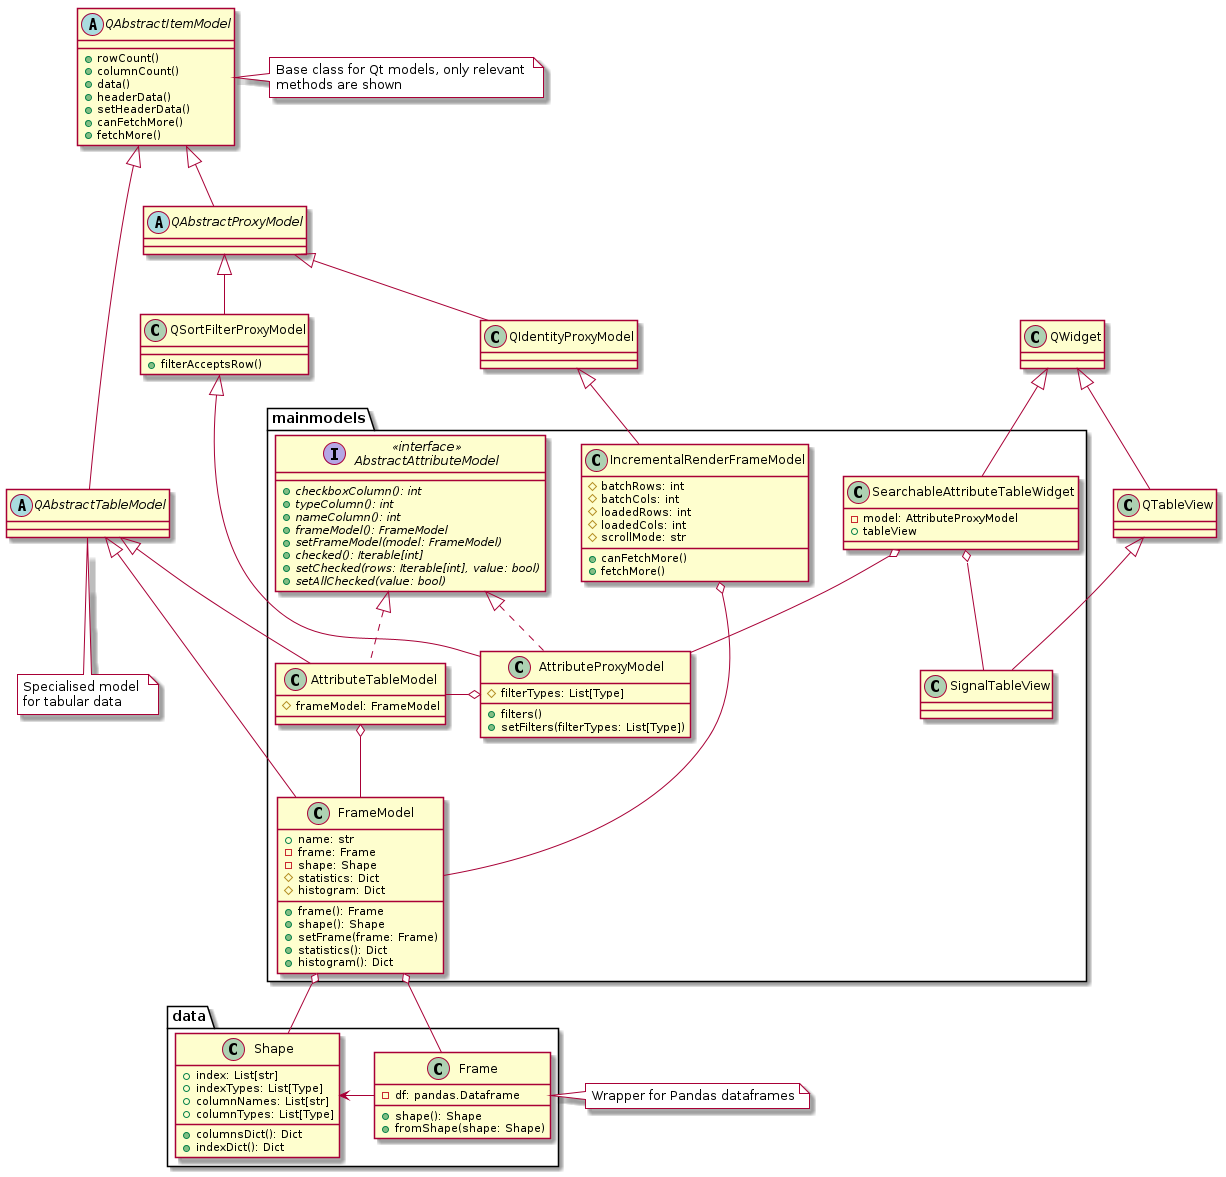
\includegraphics[width=\textwidth]{uml/models}
	\caption{Class diagram of the \texttt{mainmodels} module}
	\label{fig:modelsuml}
\end{figure}
Many classes that take part in \textit{model-view-delegate} pattern are defined inside module \texttt{gui.mainmodels}. \cref{fig:modelsuml} shows the UML class diagram for some of its classes, along with their relationship to the \texttt{data} package.\\
Qt provides specialised models and views for displaying data in many different ways: within DataMole data is often shown in tables and lists.
In order to take advantage of the Qt model-view system, model classes are required to subclass \texttt{QAbstractItemModel} and implement the relevant methods.\\
\texttt{FrameModel} handles the visualisation of the dataframe inside a \texttt{QTableView} (which is a view for tabular data).\\
\texttt{AttributeTableModel} works as a proxy model, keeping a reference to the \texttt{FrameModel} and showing only column names and types, hence is used to show the \textit{shape} of a dataset, which is required, for instance, in the \textit{Attribute panel}.\\
\texttt{AttributeProxyModel} further refines the data shown in an \texttt{AttributeTableModel} by adding filtering capabilities, like attribute search by name or regular expression and type filtering. This last feature is exploited in the operation editors that only allow the user to select the subset of columns with supported types.\\ 
When a dataset with thousands of columns or rows is visualised inside a table, the process of filling every table cell with the data from the model can take time, and the GUI would be unresponsive while this happens. Proxy class \texttt{IncrementalRenderFrameModel} solves this problem: it shows the exact same data as the \texttt{FrameModel} it proxies, but implements additional methods, specifically \texttt{fetchMore} and \texttt{canFetchMore}, to make sure the table is filled on demand, only when it is scrolled. When this happens it loads the next batch of 50 columns or 400 rows depending on the scrolling direction.\\
\texttt{SignalTableView} defines the view used to show tabular data in the program. It inherits \texttt{QTableView} capabilities and defines a customised \textit{signal} used to correctly handle rows selection and deselection. This class is used inside the \texttt{SearchableAttributeTableWidget}, a reusable widget that shows data inside a table complete with a search bar above it.\\
Finally the module also defines a custom delegate class and a custom header for the table (not shown in \cref{fig:modelsuml}), to be set in views that need to show a checkbox in one of their columns.

\clearpage
\subsubsection{The workbench}
As explained in the previous section every loaded dataframe is contained in a \texttt{Frame} object. These objects are wrapped in a \texttt{FrameModel} for visualisation inside Qt views. All these datasets are kept in the \texttt{WorkbenchModel}, the centralised container for dataframes (diagram in \cref{fig:workbench_uml}).
It provides methods to access frame models by row number (index) or name, that makes it usable as a list-like or dictionary-like container. Its \texttt{setDataframeByName} method is called whenever a new dataset, which was loaded or created by applying operations, must be added to the workbench.
The workbench is shown using its specialised view class \texttt{WorkbenchView}, which overrides some methods to allow item reordering, selection and the display of a menu on right click.
\begin{figure}
	\centering
	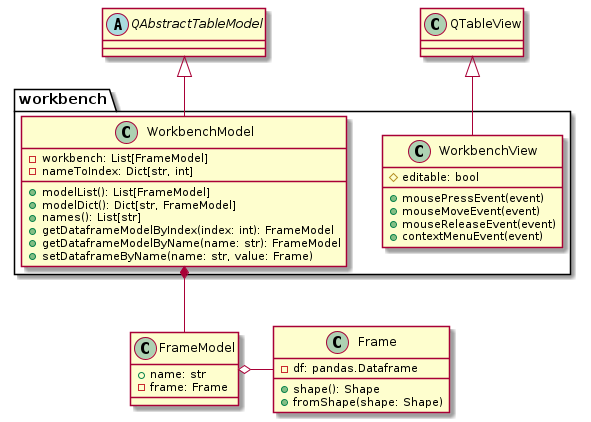
\includegraphics[width=0.8\textwidth]{uml/workbench}
	\caption{Class diagram of the \texttt{workbench} module}
	\label{fig:workbench_uml}
\end{figure} 


\subsection{Representation of a dataset transformation}
When defining a pipeline, every operation takes one or more datasets in input and produces a result that must be the input of the next transformation. Sometimes transformations must be parametrised with a variable number of arguments that represent the configuration of the operation. Additionally every transformation should be logged, in order to keep a trace of how a dataset was changed and, depending on the operation, it might be possible to undo it.\\
With these requirements it seemed convenient to implement a \textit{command pattern}: every \textit{data transformation}, also called \textit{operation} in this document, is encapsulated in a object of type \texttt{Operation}, whose contract is described in the next section. 

\subsubsection{The \textit{Operation} abstract class}
Every operation defined in DataMole is a concrete subclass of \texttt{Operation}. \cref{fig:operationuml} shows the \texttt{Operation} abstract class and its subclasses.
\begin{figure}
	\centering
	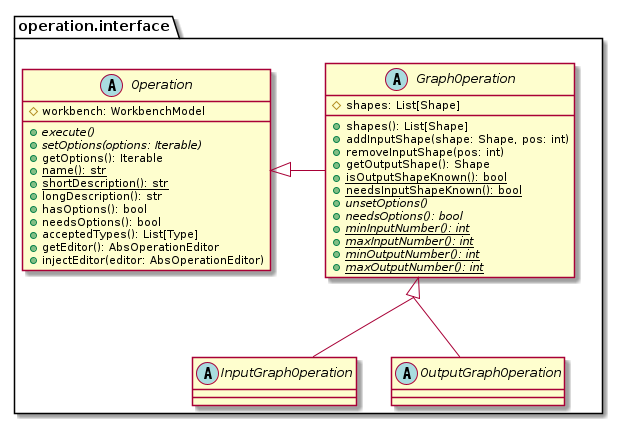
\includegraphics[width=0.8\textwidth]{uml/operation}
	\caption[Hierarchy of Operation interfaces]{Hierarchy of Operation abstract classes}
	\label{fig:operationuml}
\end{figure}

An operation keeps a reference to the workbench, which provides access to any loaded dataset. Every operation has a name, comes with a short and optionally a long description to be shown in the \textit{editor widget}. The long description is shown on user request on a separate help panel, and contains a detailed description of how the operation works and how it should be configured. \\
The \texttt{execute} method is run to apply the operation to its input arguments, which are passed as parameters.\\
The \texttt{getOptions}/\texttt{setOptions} methods are reimplemented in every operation to respectively get and set its arguments. If required, \texttt{setOptions} can also validate the new options before setting them. If they are not correct it raises an exception of type \texttt{OptionValidationError} which is handled by the controller. This mechanism is further described in §\ref{par:option_validation}.\\
Methods \texttt{hasOptions} and \texttt{needsOptions} return a boolean value depending on whether the operation is configured or needs an option editor widget. If the latter is true, the operation also needs \texttt{getEditor} to be overridden to return the widget that the operation will use to be configured. In order to avoid the definition of a new widget for every operation, an \textit{editor factory} was provided and can be used to quickly create editors with standard option fields (checkboxes, combo boxes, line edits, etc.).\\
While \texttt{getEditor} only returns a new editor widget, the \texttt{injectEditor} method is used to configure the editor.\\
Finally the \texttt{acceptedTypes} method defines which types are accepted by the operation.

\subsubsection{The editor widget factory}
Most operations require options that must be supplied by the user. For example the \texttt{KBinsDiscretizer} operation requires the user to select the columns to be discretized, specify the number of bins for every column and select the strategy to be used. To configure an operation, the widget returned by method \texttt{getEditor} is used. For most operations this widget is composed of a table with some editable columns and some radio buttons or checkboxes. To avoid code duplication and to speed up the process of creating widgets, a factory class was defined. \cref{fig:factoryuml} gives an overview of the class methods.
\begin{figure}
	\centering
	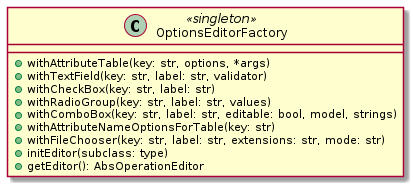
\includegraphics[width=0.6\textwidth]{uml/factory}
	\caption{Widget factory class specification}
	\label{fig:factoryuml}
\end{figure}

Factory methods allow appending widgets to the editor layout stacking them vertically, thus the order of invocation determines their ordering. The factory is a \textit{singleton} object that must be re-initialised every time it is used by invoking the \texttt{initEditor} method. This method also accepts an optional \texttt{subclass} parameter with the type of the editor to be created. This is particularly useful when an editor needs signals or slots to be part of its class definition. To give an example, \cref{fig:editor_factory} shows the editor for the \textit{Fill NaN} operation, created by calling the following factory methods:
\begin{itemize}
	\item \texttt{withAttributeTable}: this method creates widget \textit{(A)}, which is a table showing every attribute name and type, with a configurable number of extra editable columns used to receive options for every attribute. In this example the table requires the values to be filled if the option to fill by value is selected (column \textit{Fill value});
	\item \texttt{withRadioGroup}: adds a set of exclusive radio buttons and a descriptive title \textit{(B)}: in the example it is used to select the strategy for filling missing values.
\end{itemize}
Further details about the factory usage and methods configuration are reported in the next chapter, in §\ref{sssec:factory-usage}.
\begin{figure}
	\centering
	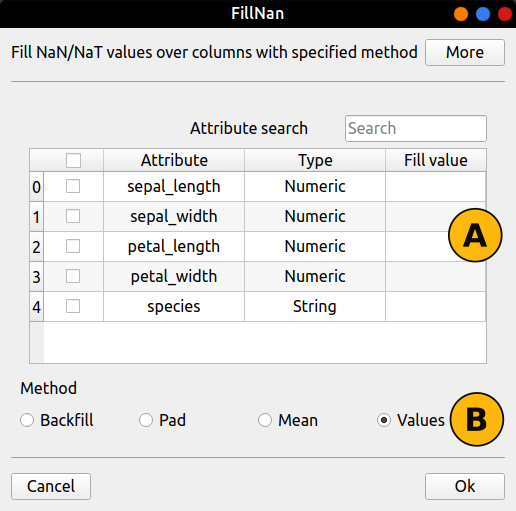
\includegraphics[width=0.6\textwidth]{editor-sample}
	\caption[Example of an \textit{option editor} created with the widget factory]{Example of an \textit{option editor} whose body widgets (\textit{A} and \textit{B}) are created with the widget factory}
	\label{fig:editor_factory}
\end{figure}

Of course not every widget can be created with the factory: complex editors with particular requirements must be defined manually. For instance, this is the case for the \texttt{Join} and \texttt{ExtractSeries} operations.

\subsection{The computational graph}
As explained in §\ref{ssec:packages}, the package \texttt{gui.graph} defines the components of the graphical user interface which allow the user to interactively create a computational graph of operations: new nodes (i.e. operations) can be added, moved, deleted and connections can be created between existing nodes to create chains of operations. Hence, this interactive flowchart can be seen as a \textit{pipeline} of data transformations, internally modelled as a \textit{directed acyclic graph}. The class diagrams of the \texttt{gui.graph} and \texttt{flow} packages are depicted in \cref{fig:daguml}.

\subsubsection{Pipeline laziness}
Whenever a new operation is added, it is not executed immediately: the pipeline is \textit{lazy}, meaning that it is evaluated completely only when the user requests it. Thus every node with an ancestor does not know its input until the whole pipeline is executed. However most operations require to be configured with additional arguments through theirs editor widgets, and often this arguments depends on the operation input (for example the user may be asked to select the columns to transform), so in order to do this they \textit{need} some information about their inputs. Additionally, every time the operation is configured, its options are validated, process that often depends on the column and index types. To solve these problems every operation needs to be able to describe some properties of its output before execution, provided a description of its inputs and the required options. Specifically, it should describe the \textit{shape} of its output. The \textit{shape} of a \texttt{Frame} object is encapsulated inside the type \texttt{Shape}: it includes information about the name and type of every column, including the ones used as dataframe index. How the dataset shape is propagated through the graph is described in the following sections.

\subsubsection{The \textit{GraphOperation} abstract class}
The additional requirements of the operations that need to execute inside the pipeline motivated the definition of the \texttt{GraphOperation} class, that specialises \texttt{Operation} adding methods only relevant in the pipeline context. Every graph operation needs to define how many inputs it needs and how many output connections it supports. This information is conveyed by the \texttt{minInputNumber}, \texttt{maxInputNumber} and their respective counterparts for the output number. \\
Moreover every graph operation reimplements method \texttt{getOutputShape}, which returns the \texttt{Shape} object describing the names and types of every column in the dataset after the application of the operation. Because this information needs to be propagated through the graph, operations also provide the \texttt{addInputShape} and \texttt{removeInputShape} methods, to manage the shapes object when some configuration changes or connections are removed.\\
However, there are situations when it might not be possible to predict the output shape before the operation is run. If this is the case, method \texttt{isOutputShapeKnown} can be redefined to return \textit{False}. This is the case for the \texttt{RemoveBijections} operation, which automatically removes every column which is a bijection of the others. Conversely some operations might not require knowing in advance the shape of the input coming from their incoming connections, in which case \texttt{needsInputShapeKnown} should be redefined to return \textit{False}. For example \texttt{RemoveNanRows}, the operation used to remove every row with a certain ratio of missing values, does not need to know the input dataset shape because its output shape does not depend on it: since the operation just remove rows, the output shape does not change at all.

\subsubsection{The graph data structure}
The operations added to a pipeline are stored inside a \texttt{DiGraph}, a data structure that models a direct acyclic graph, provided by \texttt{networkx}, a very popular network analysis library. This data structure is wrapped into an \texttt{OperationDag} object, that contains some helper functions to manage the graph of operations.\\
Before choosing to implement a simple computational graph using \texttt{networkx}, these Python libraries specific for creation and management of computational graphs were also considered:
\begin{itemize}
	\item \textbf{Luigi}: a package that simplifies the creation of pipelines of batch jobs;
	\item \textbf{GraphKit}: a library used to manage and run graph of computations (DAGs);
	\item \textbf{Dask}: this library offers many tools for scalable computations and its schedulers support the execution of customised task graphs.
\end{itemize}
Eventually we decided to avoid using such libraries, since computations in DataMole are not particularly heavy and thus would not have benefited from the advanced features provided by these packages. Additionally integrating them in a graphical interface would require much work and time, because their API is not made for this use case, but rather for usage in Python scripts.

\subsubsection{The GUI for the graph}
GUI components used to manage the graph are defined in the \texttt{gui.graph} sub-package.
This package makes use of the \textit{Qt Graphics View Framework}, the Qt module for efficient rendering and management of graphic items \cite{site:qt-doc-graphics-view}. Many modules of this package were adapted from \cite{site:nodegraph-pyqt}, a project that used Python and Qt to build a generic graph manager, and is licensed under GNU GPL.

\lineparagraph{Main graphic components}
The \textit{Qt Graphics View Framework} relies on three main classes:
\begin{itemize}
	\item \texttt{QGraphicsItem}: represents a graphic item that can be shown within a graphics scene;
	\item \texttt{QGraphicsScene}: the scene manages all the graphic items and provides functionality to efficiently determine items location, and control zooming and selection;
	\item \texttt{QGraphicsView}: visualises the content of a \texttt{QGraphicsScene}.
\end{itemize}
\cref{fig:daguml} shows the classes defined in the \texttt{gui.graph} package. All graphical items are contained in the \texttt{GraphScene} a subclass of \texttt{QGraphicsScene} that additionally handles drag-and-drop actions and mouse events. Graph \textit{nodes} and \textit{edges} are respectively drawn using the \texttt{Node} and \texttt{Edge} classes, both subclasses of \texttt{QGraphicsItem}. Every \texttt{Node} has a unique id that matches the id of the operation it represents. The \texttt{NodeSlot} item is used to draw the circular sockets that represent the operation inputs and outputs and are used to create connections. Finally \texttt{RubberBand} is used to handle mouse selection.\\
A \textit{controller}, modelled by class \texttt{GraphController}, is used to ensure that the graphic interface is kept synchronized with the underlying data structure containing the graph. Every graph node is an object of type \texttt{OperationNode} which wraps a \texttt{GraphOperation} and adds some helper methods used to manage pipeline nodes.
\begin{figure}
	\centering
	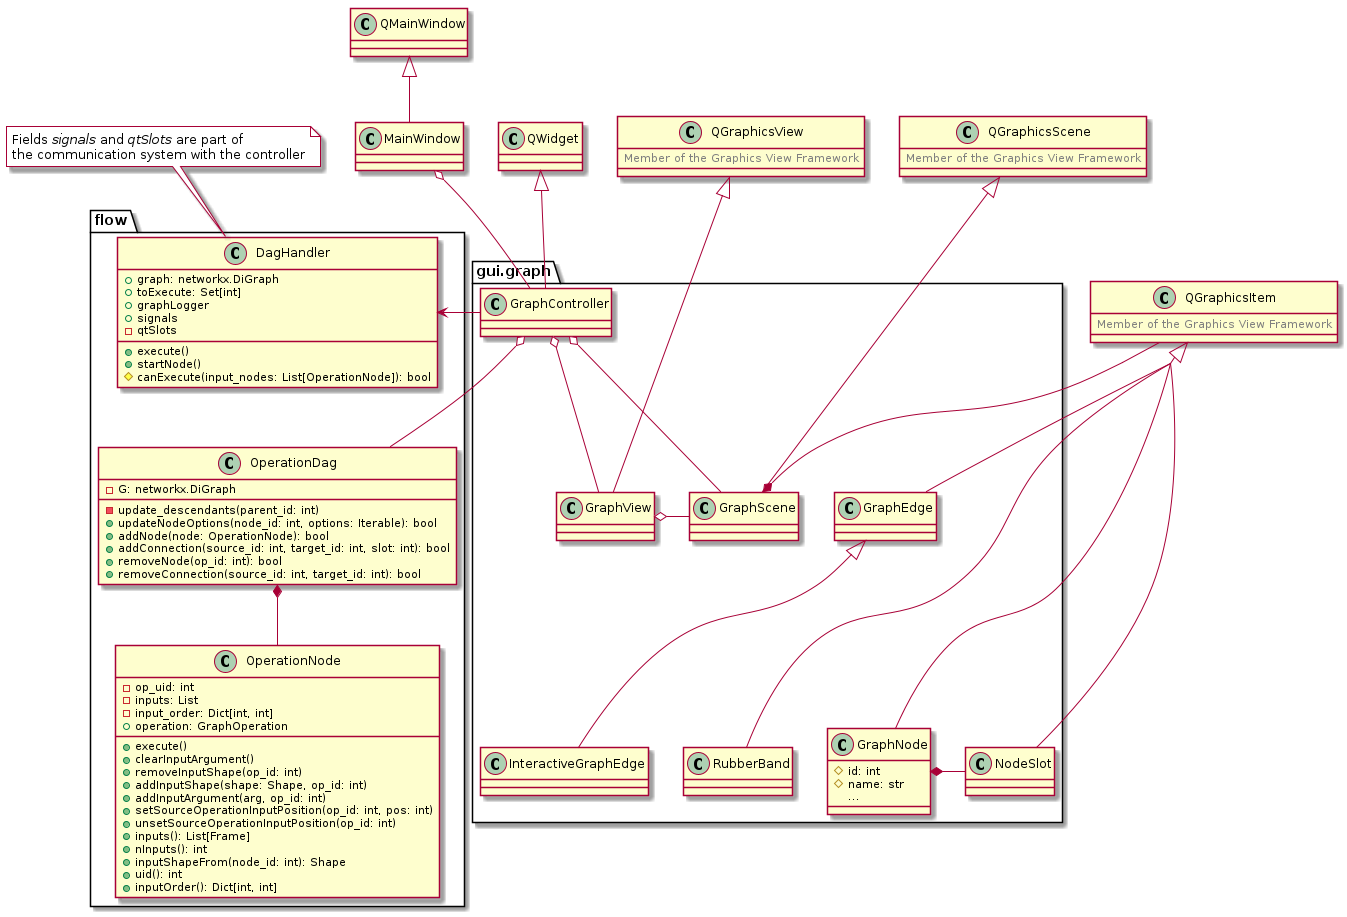
\includegraphics[width=\textwidth]{uml/dag}
	\caption{Class diagram of the \texttt{gui.graph} and \texttt{flow} packages}
	\label{fig:daguml}
\end{figure}

\subsubsection{Pipeline management workflow}\label{sssec:pipeline-sequence}
The \texttt{GraphController} interprets the user actions on the view and keeps updated the graph data structure inside the \texttt{OperationDag} object. This section describes how the controller and the other classes interact with each other to manipulate the pipeline.

\lineparagraph{Node creation}
Nodes are placed on the graphic scene with drag-and-drop, by selecting operations from a list and dropping them on the graphic view. When a new operation is dropped, method \texttt{dropEvent} of \texttt{GraphScene} is called and the \textit{scene} invokes method \texttt{getDropData} to retrieve the type of the operation that was dropped. It then emits a signal to ask the \textit{controller} to manage the creation of the new operation. The controller instantiates the new \texttt{Operation} and \texttt{OperationNode} objects, updates the graph with the new operation and, if successful, it updates the graphic scene with the new node. This entire process is depicted with the sequence diagram in \cref{fig:add_node_seq}.
\begin{figure}
	\centering
	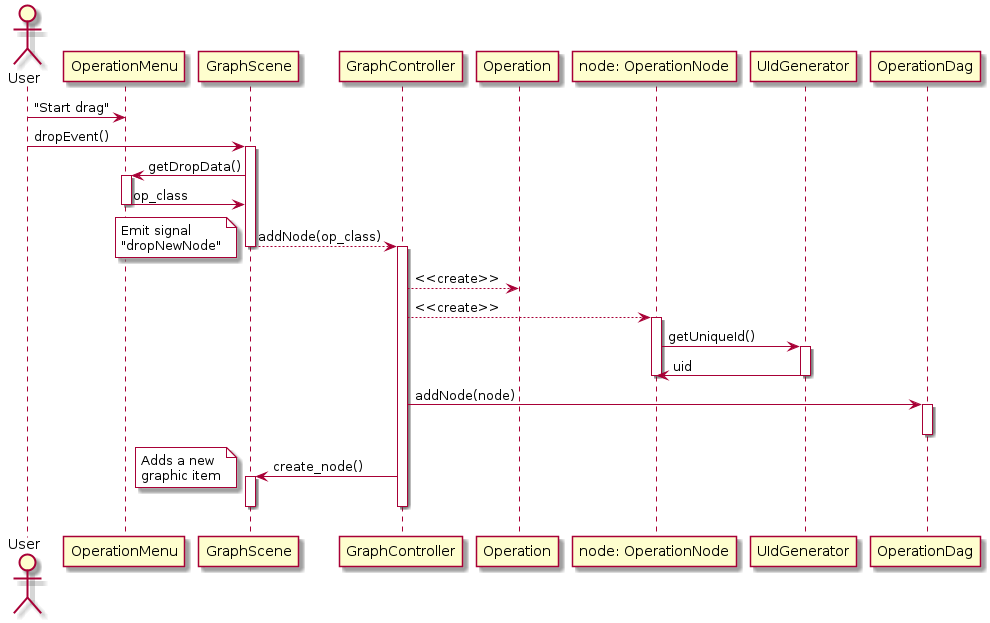
\includegraphics[width=\textwidth]{uml/operation_add}
	\caption{Sequence diagram describing the creation of a new pipeline node}
	\label{fig:add_node_seq}
\end{figure}
On the other hand, if something goes wrong and the pipeline cannot be updated, the controller shows an error message and nothing is changed.

\lineparagraph{Edge creation}
When the user starts to drag a new edge from a \texttt{Node}, it emits a signal and causes the \texttt{start\_interactive\_edge} method of the \textit{scene} to be called. Its purpose is to display an interactive draggable edge that exits the source node and follows the mouse pointer until the user drops its head on the target node. When this happens \texttt{stop\_interactive\_edge} is called. This method looks for a free node slot in the target node. If a free slot is found the \texttt{addEdge} method of the \textit{controller} is called to update both the acyclic graph and the graphic view accordingly. The corresponding sequence diagram is shown in \cref{fig:add_edge_seq}. \\
If the edge cannot be added, for example because the source operation does not provide an input shape which is needed by the target operation, an error message is shown to the user. In either case the temporary \texttt{InteractiveEdge} object created to display the draggable edge is eventually deleted.
\begin{figure}
	\centering
	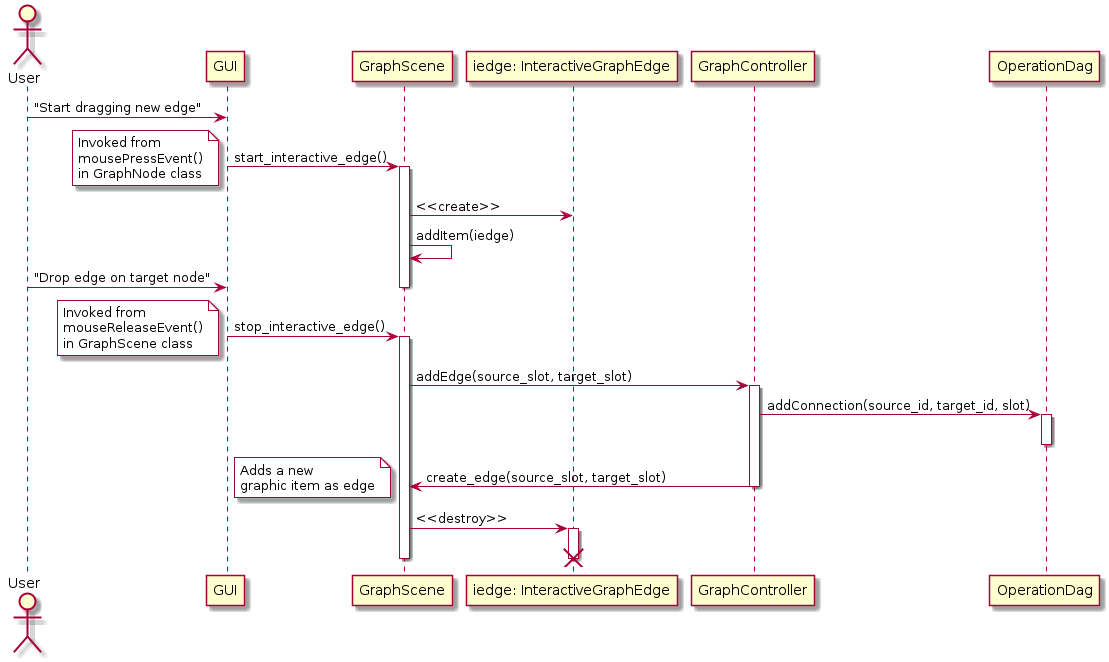
\includegraphics[width=\textwidth]{uml/connection_add}
	\caption{Sequence diagram for connecting two existing operations}
	\label{fig:add_edge_seq}
\end{figure}

\lineparagraph{Operation configuration}
\label{par:operation_config}\noindent
Double clicks on existing operations cause the editor widget to be shown. \cref{fig:operation_config_sequence} describes how the widget is created and configured. First the \textit{controller} retrieves the \texttt{Operation} object corresponding to the clicked item using its unique id. Afterwards the editor is created using the \texttt{getEditor} method and the existing options are retrieved from the operation and set into the editor widget. Finally the editor is configured with the \texttt{injectEditor} invocation and shown to the user.
\begin{figure}
	\centering
	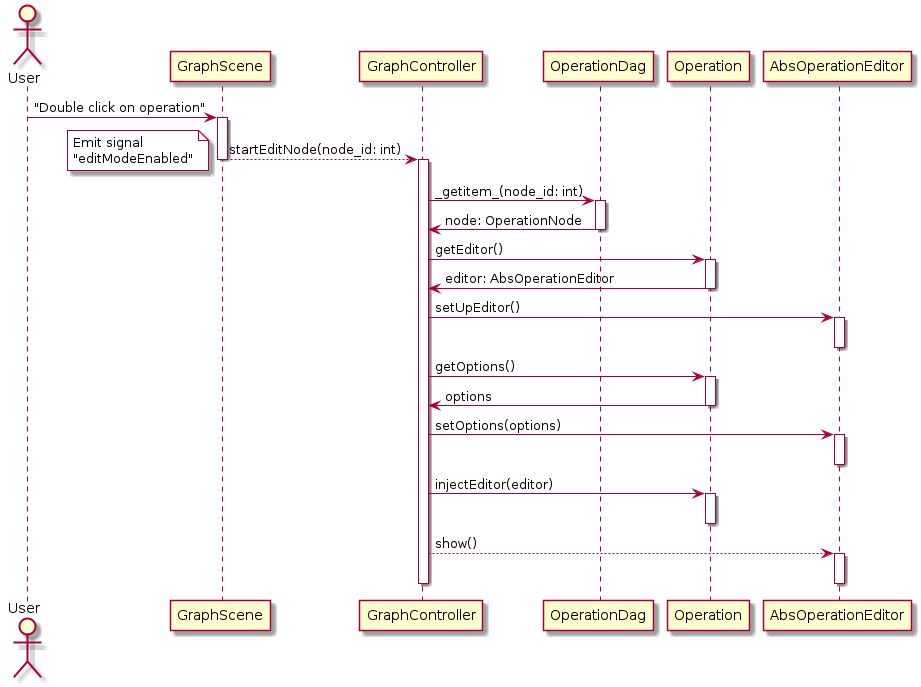
\includegraphics[width=\textwidth]{uml/operation_config}
	\caption{Sequence diagram for operation configuration}
	\label{fig:operation_config_sequence}
\end{figure}

\lineparagraph{Option confirmation}
\begin{figure}[htbp]
	\centering
	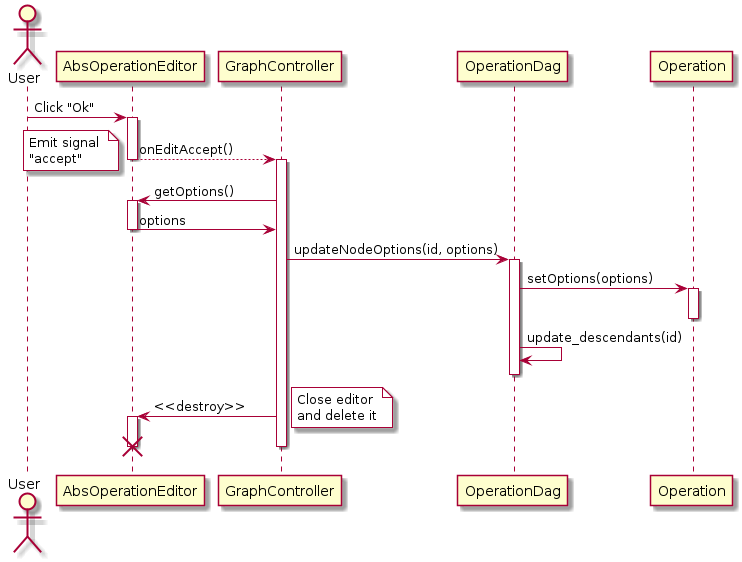
\includegraphics[width=\textwidth]{uml/controller_accept}
	\caption[Sequence of operations after options confirmation in the editor]{Sequence of operations after options confirmation assuming no validation errors occur}
	\label{fig:controller_accept}
\end{figure}
\begin{figure}[htbp]
	\centering
	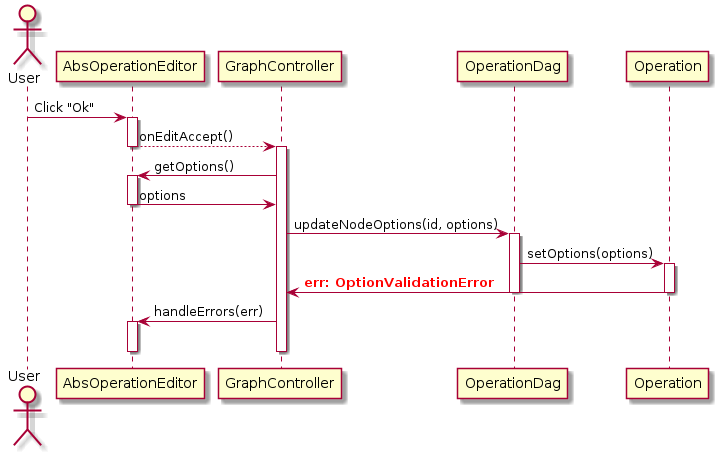
\includegraphics[width=\textwidth]{uml/controller_error_handling}
	\caption{Sequence of operations after options validation exception}
	\label{fig:controller_error_handling}
\end{figure}
Once the user sets new options in the configuration widget and confirms them, the \texttt{accept} signal is emitted by the editor. This signal is handled by the \texttt{GraphController} that retrieves the options from the editor and updates the corresponding operation. Finally the \texttt{update\_descendants} routine is run to propagate the new shape through the graph. The whole process is shown in \cref{fig:controller_accept}.

\lineparagraph{Option confirmation with validation errors}\label{par:option_validation}\noindent
The \texttt{setOptions} method defined in every operation can raise an exception of type \texttt{OptionValidationError} if one or more options are not correct and need to checked by the user. This exception is parametrised with a list of tuples, where each one represents an error, with a key and an error message for the user. After the user confirms the options in the configuration widget, eventual validation errors are notified inside the editor window. The process leading to this outcome is outlined in \cref{fig:controller_error_handling}.\\
Error messages are normally shown on the bottom of the editor widget. If a more advanced error handling is required, it is possible to change this behaviour by defining custom error handling functions. This is detailed in §\ref{ssec:define-editor}.

\subsubsection{Executing the pipeline}\label{sssec:pipeline-execute}
Execution of the pipeline is handled by the \texttt{DagHandler} class. This handler is instantiated by the controller to direct the execution of the whole pipeline. First it checks for runnable operations: an operation is considered \textit{runnable} if all the required options and its input dataframes are set. Starting from the input nodes, runnable operations are scheduled for execution on a separate thread. When an operation completes, its output is set as the input of all its successors and all runnable operations are started.\\
Additionally the handler communicates with the controller emitting a specific signal when the status of an active operation changes (i.e. if it is running, has completed with error, etc.). This allows the controller to update the status of each node in the graphic view.

\lineparagraph{Multithreaded execution}
In a Qt application, all QWidgets run in the \textit{main thread}, also called the \textit{GUI thread} \cite{site:qt-threading-gui}. If a time-expensive computation is run on this same thread the GUI will freeze and stop responding until the operation completes. To avoid this problem every operation to be executed is wrapped inside a \texttt{QRunnable} object and is added to a \texttt{QThreadPool} for execution. The combined usage of \texttt{QRunnable} and \texttt{QThreadPool} represents a simple multithreading pattern in Qt, with the advantage that the \texttt{QThreadPool} takes care of thread management, including their creation and destruction: it creates a predefined number of threads equal to the number of cores of the machine and reuses them whenever a new operation is added to the pool. Considering that thread creation and destruction can be costly, this pattern provides an higher-level alternative to thread management with the \texttt{QThread} class, which would instead create a new thread every time, without reusing them \cite{site:qt-threading-reuse}.\\
The helper class \texttt{Worker} was defined in the \texttt{threads} module, and is shown in \cref{fig:threads_module}.
\begin{figure}
	\centering
	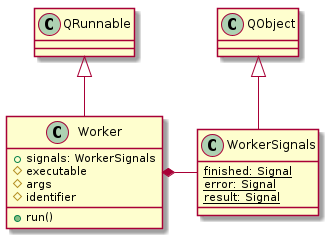
\includegraphics[width=0.6\textwidth]{uml/threads}
	\caption{Class diagram of the \texttt{threads} module}
	\label{fig:threads_module}
\end{figure}
\texttt{Worker} objects wrap \textit{executable objects}, which are arbitrary Python objects that define an \texttt{execute} method (like \texttt{Operation} instances). The worker is provided the list of arguments that should be passed to the \texttt{execute} method, if any, and an \texttt{identifier} to be used when a signal is emitted.
A \texttt{WorkerSignal} class inheriting \texttt{QObject} is defined because \texttt{QRunnable} does not inherit \texttt{QObject} and thus can not emit signals. 
Through this class, workers emit three signals, depending on their state:
\begin{itemize}
	\item \textit{error}: this signal is emitted then the worker was running the operation but a runtime error occurred. The signal arguments are the operation identifier and the error information;
	\item \textit{result}: emitted then the operation completes successfully. It carries the operation result (i.e. the return value of the \texttt{execute} method) and the operation identifier;
	\item \textit{finished}: signal emitted immediately before the \texttt{run} method of the worker returns, and carries the identifier.
\end{itemize}
These signals provide a way to monitor the status of every operation and are used by the \texttt{GraphController} to update the graphic view.

\lineparagraph{Considerations and alternatives}
The \texttt{QRunnable} and \texttt{QThreadPool} pattern is a very simple multithreading pattern, and indeed was chosen for its simplicity. By comparison, the \texttt{QThread} class provides much more flexibility, at the cost of explicitly managing threads. The main drawback of the selected approach is the lack of support for stopping a running operation. This comes from the fact that \texttt{QThreadPool} does not expose the underlying threads and thus stopping them becomes impossible.\\
On the other hand, an equivalent approach using \texttt{QThread} may involve defining a customised thread pool that keeps track of the running threads, in order to terminate their execution when required. Nonetheless, caution is required when stopping a running thread as it may leave data in an inconsistent state.\\
Using the Qt Concurrent module would be a simpler alternative: this module, part of the Qt Framework, provides high-level functions to deal with some common parallel computation patterns \cite{site:qt-concurrent}. Unfortunately this module is not included in the Python bindings for Qt. That is because the Qt Concurrent heavily relies on C++ templates and due to the Python dynamically-typed nature and the impossibility of generating C++ code at runtime there is not way to generate the Python bindings.

\subsection{The \textit{OperationAction} controller}
\begin{figure}
	\centering
	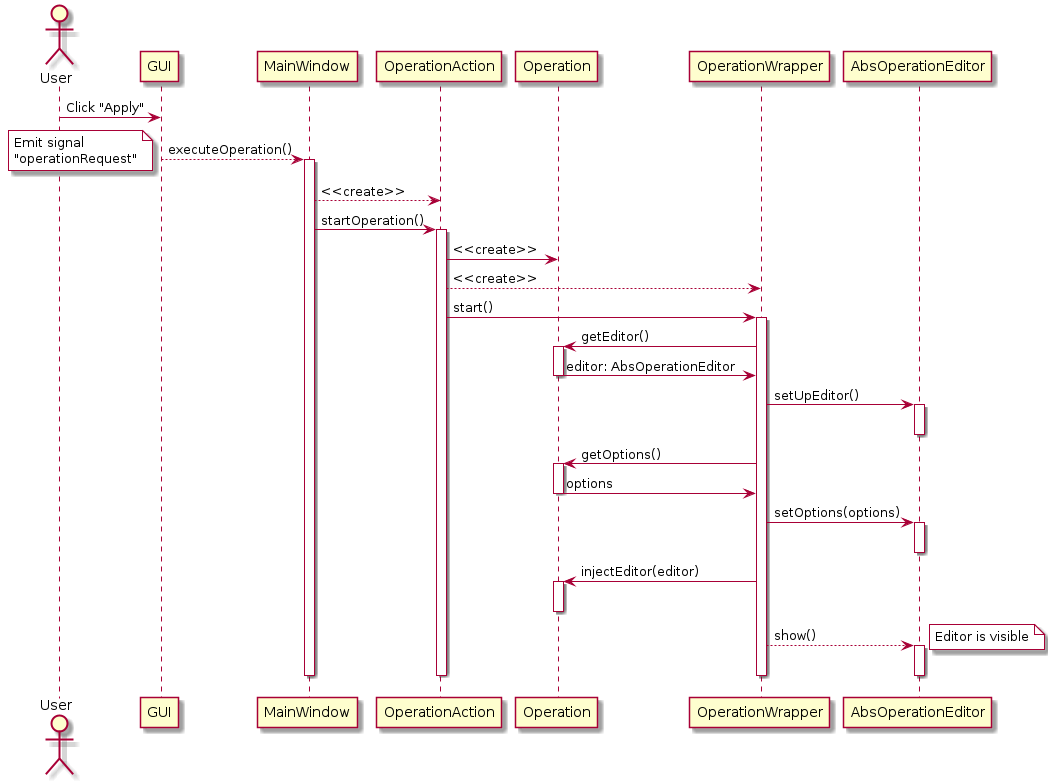
\includegraphics[width=\textwidth]{uml/actionwrapper_apply}
	\caption{Sequence diagram of editor creation and display}
	\label{fig:actionwrapper_apply_seq}
\end{figure}
\begin{figure}
	\centering
	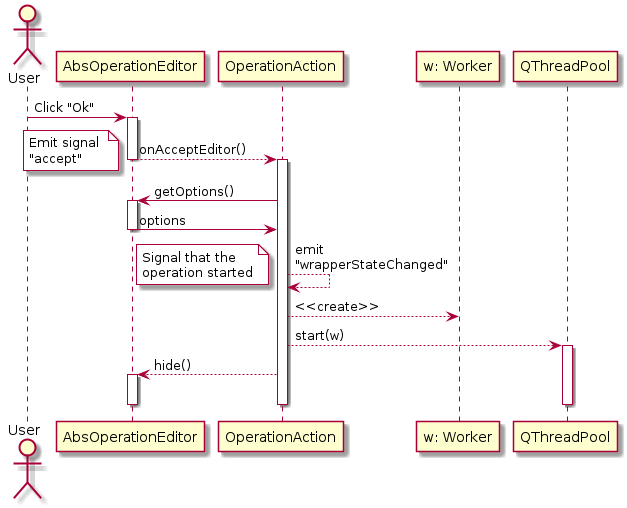
\includegraphics[width=0.85\textwidth]{uml/actionwrapper_confirm}
	\caption{Sequence diagram of the option confirmation process}
	\label{fig:actionwrapper_confirm_seq}
\end{figure}
\begin{figure}
	\centering
	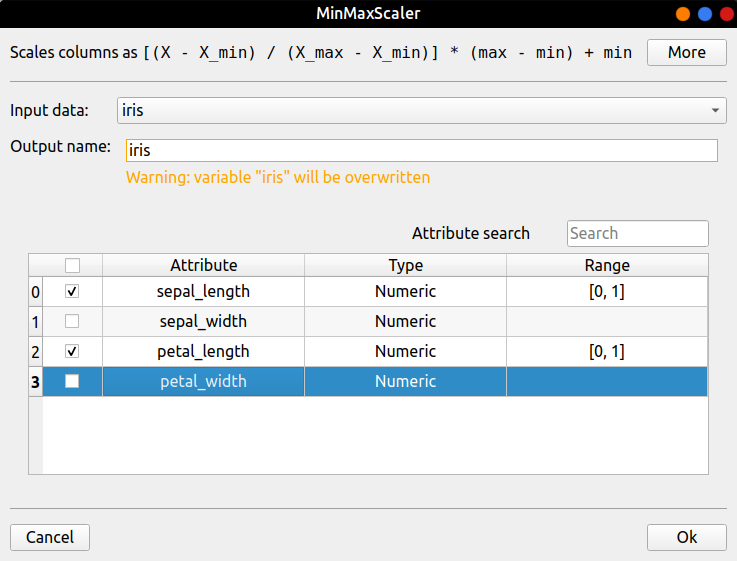
\includegraphics[width=0.7\textwidth]{interface/editor_image}
	\caption[The editor widget for min-max scaling]{The editor widget for min-max scaling. The editor is also warning the user that the output name already exists in the workbench, and thus the output of the operation will overwrite the current dataset.}
	\label{fig:editor_widget}
\end{figure}
A controller class named \texttt{OperationAction} was designed to manage the application of operations from the \textit{Attribute panel}. This class inherits \texttt{QAction} which provides the support for launching operations from menu bars.\\ 
An \texttt{OperationAction} wraps an \texttt{Operation} and when \textit{triggered}, either explicitly or implicitly (e.g. by clicking an action in a menu), it shows the option editor and waits for the user to set them. The whole process is described with a sequence diagram in \cref{fig:actionwrapper_apply_seq}.  After confirmation, if validation succeeds the operation is executed: to do this a \texttt{Worker} object is created and added to the \texttt{QTreadPool} global instance. The sequence diagram for this is shown in \cref{fig:actionwrapper_confirm_seq}.
If option validation fails, errors are shown as already discussed in §\ref{par:option_validation}.\\
Because every \texttt{GraphOperation} is also an \texttt{Operation}, the \texttt{OperationAction} wrapper can also run graph operations as single commands, outside of the graph context. To execute such an operation as a single command there are two additional options that the user must provide: the input dataset and a name for the output. However editor widgets for graph operations do not provide a functionality to ask for these parameters. Consequently, whenever a graph operation is triggered, the \texttt{OperationAction} controller is also responsible of adding a combo box and an editable text box to the operation editor, before every other widget. The result can be seen in \cref{fig:editor_widget}. The combo box allows to choose which dataset to operate on and the text box requires the name of the output dataset, that will be set on the workbench when the operation completes.

\subsection{Charts visualisation}
DataMole includes some visualisation features: it can show a frequency histogram to represent value distribution, a scatterplot matrix to visualise bivariate relations and a line chart for temporal series. \\
Implementing these features required some research about existing plotting libraries that could be embedded in this project, and they are reported in the next section.

\subsubsection{Technological considerations}
All charts in the program are drawn using QtCharts. This is the official module for creating graphs within Qt and is included in the PySide2 Python package, so no additional packages are needed. It builds upon the Graphics View framework and it is quite simple to use. On the other hand, it does not provide many advanced features, and its documentation is a bit lacking, with respect to the rest of the framework.\\
The following list contains a description of other packages that can be used to plot charts inside a Qt application:
\begin{itemize}
	\item \textbf{PyQtGraph}: a scientific library based on Qt4 and \texttt{numpy}. It relies on the Qt GraphicsView framework and is released under MIT license;
	\item \textbf{QCustomPlot}: a Qt-based C++ widget for plotting and data visualisation released under GPL v3 license
	\item \textbf{PyQwt}: another plotting library for Python based on PyQt.
\end{itemize}
PyQtGraph should be considered for future extension, since it is actively maintained and works with both PyQt and PySide2. It offers many advanced features that would require much work with the official QtCharts. On the other hand, QCustomPlot does not work with PySide2 and PyQwt is not maintained anymore, and only supports older versions of Qt.

\subsubsection{The plotting package}
\begin{figure}
	\centering
	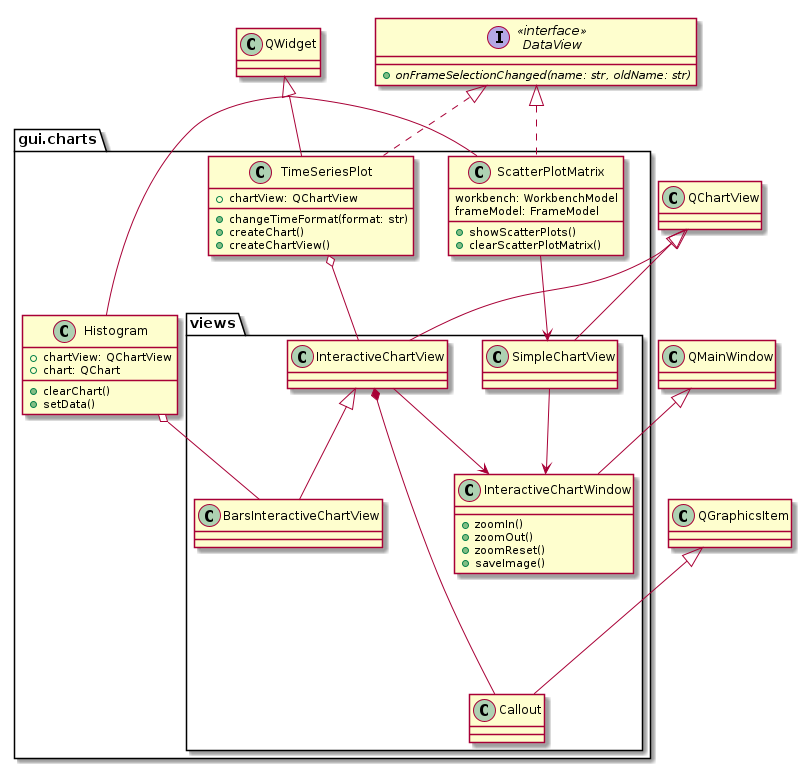
\includegraphics[width=\textwidth]{uml/charts}
	\caption{Class diagram of the \texttt{gui.charts} package}
	\label{fig:chartsuml}
\end{figure}
Package \texttt{gui.charts} defines the widgets for creating and showing plots. Additionally customised chart views are defined inside the \texttt{views} module, and some related helper functions are in the \texttt{utils} module. \cref{fig:chartsuml} shows the package class members.\\
When a chart view is double clicked the chart is copied on a secondary window, of type \texttt{InteractiveChartWindow}. This feature provides a way to move the charts around the screen as independent windows, and adds the ability to save its content as image. This feature relies on the ability to copy the chart data into a new one. Unfortunately this is not possible for the histogram chart, due to a limitation in the QtCharts module, and for this reason the \texttt{BarsInteractiveChartView} does not allow to open the chart on a new window. The \texttt{InteractiveChartView} also draws a pop-up item showing the data coordinates or label when one of its point is hovered with the cursor. This is implemented in the \texttt{Callout} class, which was inspired from the official Qt example available at \cite{site:qt-example-callout}.\\
\texttt{TimeSeriesPlot} and \texttt{ScatterPlotMatrix} are the widgets shown in the \textit{View panel}, used to create the line chart for time series and the scatterplot matrix. Every widget that adds a visualisation feature to this panel must realise the \texttt{DataView} interface. It only requires the definition of one \textit{slot},  which is called whenever the user clicks on a different dataframe in the workbench.

\subsection{Logging}
The \texttt{flogging} package provides all the logging functionalities for DataMole and internally uses the Python \texttt{logging} module. This package is used to create three different logs:
\begin{itemize}
	\item \textbf{Application log}: contains all the application messages, like warnings, errors and debug messages. These logs are dumped inside the \texttt{logs/app} folder and are mainly useful for debugging;
	\item \textbf{Operation log}: logs the operations applied directly from the \textit{Attribute panel}. Every log file is created inside the \texttt{logs/operations} folder and contains a summary of every operation run during a program session;
	\item \textbf{Graph log}: logs the execution of a pipeline. A different file is created every time a pipeline is executed inside the \texttt{logs/graph} folder.
\end{itemize}
Additionally the \texttt{logging} module also creates a root logger which logs everything passed to any active logger. This logger output is redirected inside the \texttt{logs/root} folder.

\subsubsection{Logging operations}\label{sssec:logging}
\begin{figure}
	\centering
	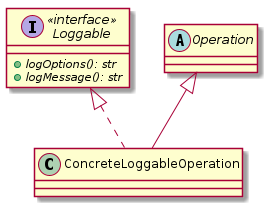
\includegraphics[width=0.5\textwidth]{uml/logging}
	\caption{Class diagram for a sample operation that can be logged}
	\label{fig:loguml}
\end{figure}
Every operation supports logging. Operations log their options configuration and every parameter set by the user.\\
Every operation that needs to be logged implements the \texttt{Loggable} interface. Diagram in \cref{fig:loguml} shows its two methods:
\begin{itemize}
	\item \texttt{logOptions}: returns a formatted string with the configuration of the operation (typically user options) or other things that can be logged before the operation is run;
	\item \texttt{logMessage}: returns a string with everything that should be logged after the operation completes, possibly including execution details.
\end{itemize}

Every time a pipeline is run the \texttt{OperationHandler} creates a new log file and logs the operations while they are executed. Operations launched from the \textit{Attribute panel} are instead logged by the \texttt{OperationAction} controller. In either case, only operations realising the \texttt{Loggable} interface are logged.

\section{Testing}
Every operation defined in DataMole has been tested to ensure that input data are always treated correctly and produce a correct output. The \texttt{Pytest} package has been used to create test suites since it is very easy to use and require no boilerplate code. Every test suite is defined in a separate file inside the \texttt{tests} folder. Every operation is tested to ensure that every accepted data type with any possible combination of options is handled as expected and that exceptions are thrown when invalid options are set.\\
Module \texttt{mocks} contains the \textit{mock class} definition for the \texttt{WorkbenchModel} and the \texttt{FrameModel} class. This is necessary because they are both subclasses of the Qt model classes, and thus they cannot be instantiated outside of a Qt Application, which is not initialised for testing purposes.\\
These unit-tests have been essential to define operations that correctly operate with Pandas and Scikit-learn. In addition, the \texttt{OperationDag} methods are tested to ensure that the graph data structure is updated correctly.\\
GUI components were not tested. To do this it may be worth using \texttt{pytest-qt} \cite{sw:pytest-qt}, a Pytest plug-in that allows to simulate user interaction to test widgets.




